\section[Фигура 1]{Фигура 1}
Строим квадрат, трижды дублируем. 
Матрицы афинных преобразований для построения правой грани куба:
\begin{equation*}
    A = 
    \begin{pmatrix}
        0.353&  1& 0\\
        0&  1& 0\\
        0&  0& 1
    \end{pmatrix} \hspace{24pt}
    B = 
    \begin{pmatrix}
        1&  0& 0\\
        1&  1& 0\\
        0&  0& 1
    \end{pmatrix} \hspace{24pt}
    C = 
    \begin{pmatrix}
        1&  0& 100\\
        0&  1& 0\\
        0&  0& 1
    \end{pmatrix}
\end{equation*}

Результирующая матрица построения правой грани куба:
\begin{equation*}
    M = C\times B\times A =
    \begin{pmatrix}
        0.353&  0& 100\\
        0.353&  1& 0\\
        0&  0& 1
    \end{pmatrix}
\end{equation*}
\vspace{12pt}

Матрицы афинных преобразований для построения верхней грани куба:
\begin{equation*}
    A_{1} = 
    \begin{pmatrix}
        1&  0& 0\\
        0&  0.353& 0\\
        0&  0& 1
    \end{pmatrix} \hspace{24pt}
    B_{1} = 
    \begin{pmatrix}
        1&  1& 0\\
        0&  1& 0\\
        0&  0& 1
    \end{pmatrix} \hspace{24pt}
    C_{1} = 
    \begin{pmatrix}
        1&  0& 0\\
        0&  1& 100\\
        0&  0& 1
    \end{pmatrix}
\end{equation*}

Результирующая матрица построения верхней грани куба:
\begin{equation*}
    N = C_{1}\times B_{1}\times A_{1} =
    \begin{pmatrix}
        1& 0.353& 0\\
        0& 0.353& 100\\
        0&  0& 1
    \end{pmatrix}
\end{equation*}
\vspace{12pt}

\newpage
Ниже приведены этапы применения изменений:
\hspace{0pt}
\begin{figure}[H]
    \begin{minipage}[h]{0.25\linewidth}
        \center{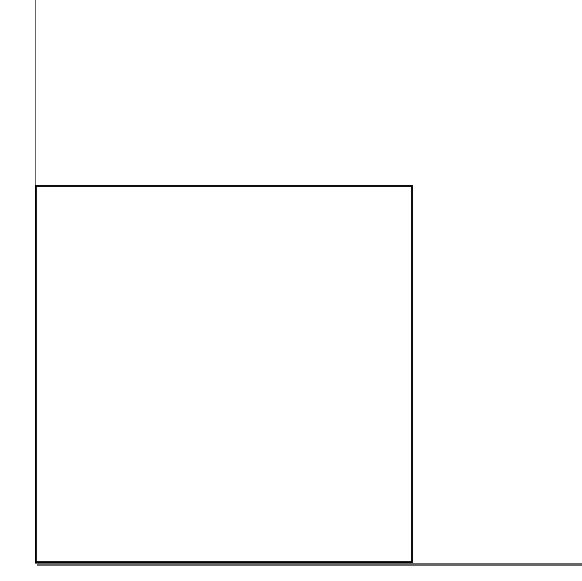
\includegraphics[width=1\linewidth]{1_1_create.png}}\\
        Создание фигур
    \end{minipage}
    \hfill
    \begin{minipage}[h]{0.25\linewidth}
        \center{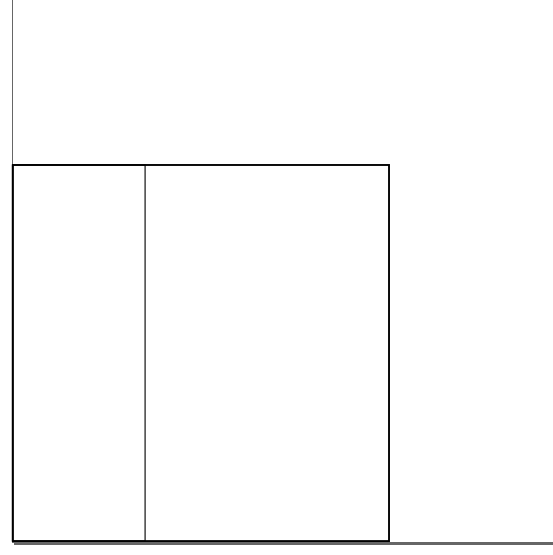
\includegraphics[width=1\linewidth]{1_2_scale.png}}\\
        Применение преобразований матрицы A
    \end{minipage}
    \hfill
    \begin{minipage}[h]{0.25\linewidth}
        \center{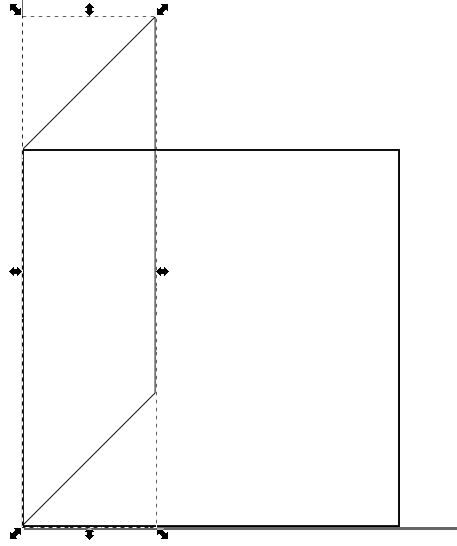
\includegraphics[width=1\linewidth]{1_3_skew.png}}\\
        Применение преобразований матрицы B
    \end{minipage}
    \vfill
    \vspace{12pt}
    \begin{minipage}[h]{0.47\linewidth}
        \center{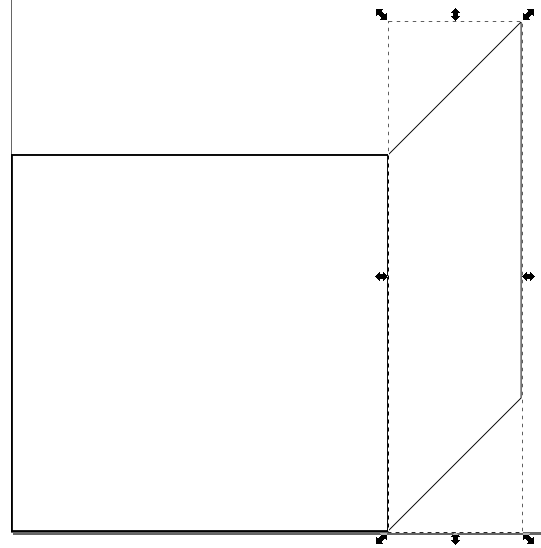
\includegraphics[width=1\linewidth]{1_4_move.png}}\\
        Применение преобразований матрицы C.\\
        Завершение построения правой грани
    \end{minipage}
    \hfill
    \begin{minipage}[h]{0.47\linewidth}
        \center{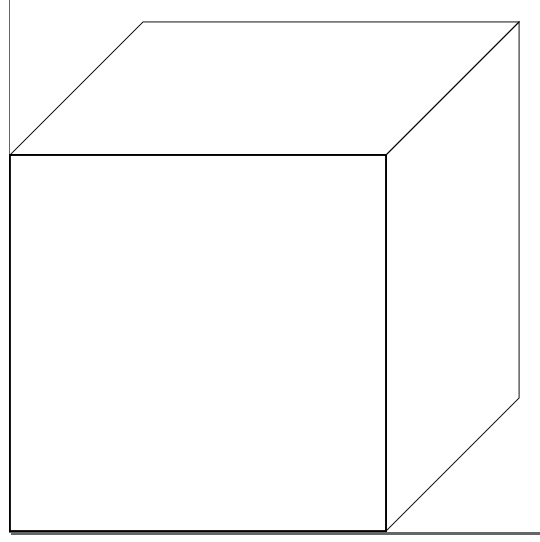
\includegraphics[width=1\linewidth]{1_5_result.png}}\\
        Применение марицы N.\\
        Завершение построения верхней грани. Завершение построения фигуры
    \end{minipage}

\end{figure}
